\chapter{Opening the black box: analyzing the learned music representation}\label{sec:model-analysis}
% **************************** Define Graphics Path **************************
\ifpdf
    \graphicspath{{Chapter5/Figs/Raster/}{Chapter5/Figs/PDF/}{Chapter5/Figs/}}
\else
    \graphicspath{{Chapter5/Figs/Vector/}{Chapter5/Figs/}}
\fi

A common criticism of deep learning methods are their lack of interpretability,
an area where symbolic rule-based methods particularly excel. In this section,
we argue the opposite viewpoint and demonstrate that characterization of the
concepts learned by the model can be surprisingly insightful. The benefits of
cautiously avoiding prior assumptions pay off as we discover the model itself learns
musically meaningful concepts without any supervision.

\section{Investigation of neuron activation responses to applied stimulus}

Inspired by stimulus-response studies performed in neuroscience, we choose to
characterize the internals of our sequence model by applying an analyzed music
score as a stimulus and measuring the resulting neuron activations. Our aim
is to see if any of the neurons have learned to specialize to detect musically meaningful
concepts.

We use as stimulus the music score shown in \cref{fig:model-analysis-stimulus},
which has already been preprocessed as described in \vref{sec:preprocessing}.
To aid in relating neuron activities back to music theory, chords are annotated
with Roman numerals obtained using {\tt music21}'s automated analysis. Note
that Roman numeral analysis involves subjectivity, and the results of automated
analyses should be carefully interpreted.

\begin{figure}[p]
    \centering
    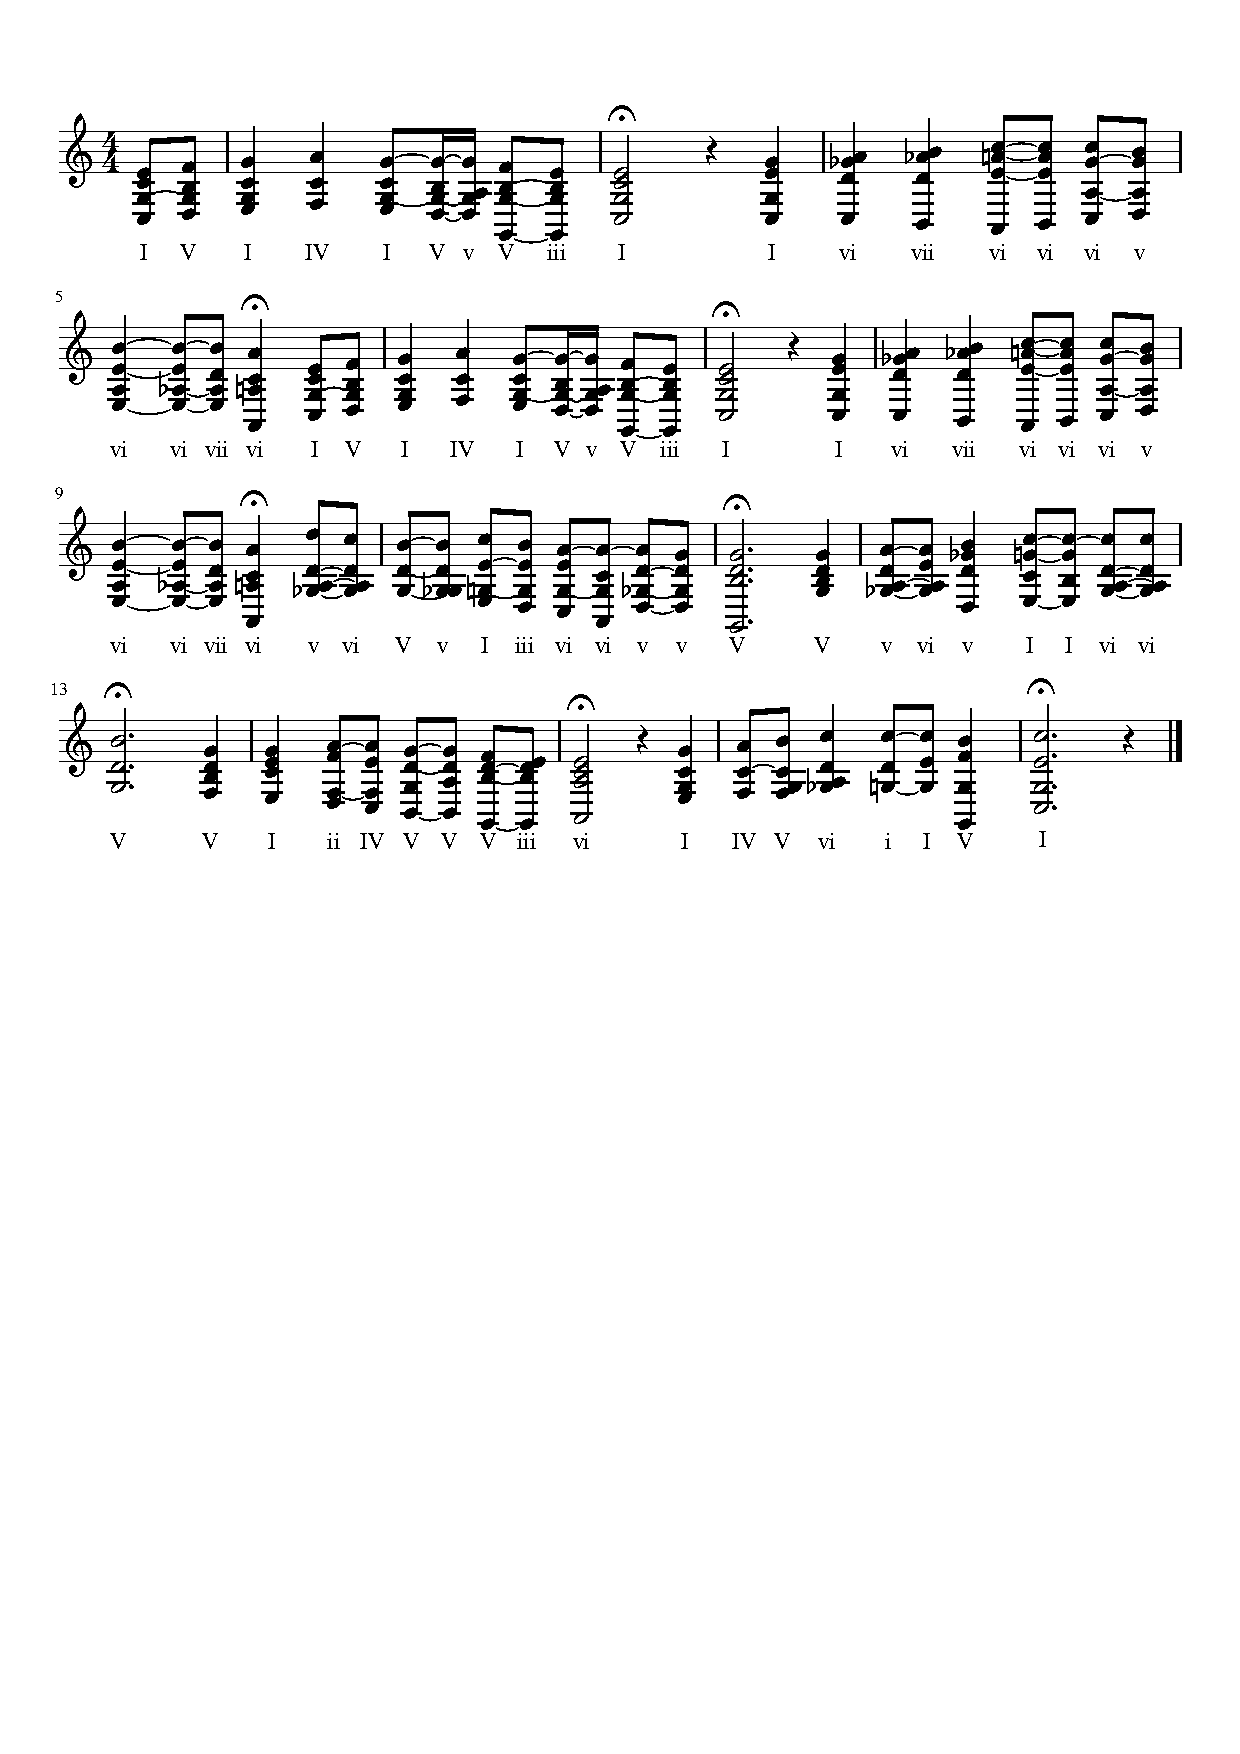
\includegraphics[trim={0 15cm 0 0},clip,width=0.9\linewidth]{model-analysis-input-score.pdf}
    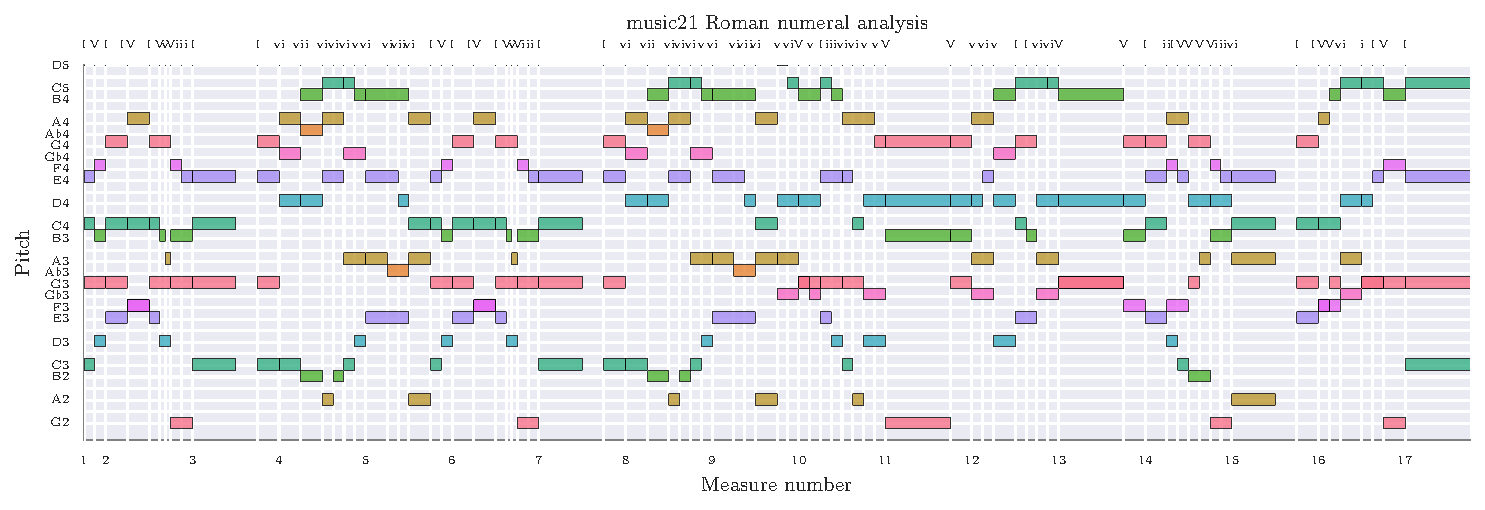
\includegraphics[width=1.00\linewidth]{model-analysis-input-piano-roll.pdf}
    \caption{{\it Top}: The preprocessed score (BWV 133.6) used as input stimulus with Roman numeral analysis annotations obtained
        from {\tt music21}; {\it Bottom}: The same stimulus represented on a piano roll}
    \label{fig:model-analysis-stimulus}
\end{figure}

\subsection{Pooling over frames}

In order to align and compare the activation profiles with the original score,
all the activations occuring in between two chord boundary delimiters must be
combined. This aggregation of neuron activations from higher resolution (\eg
note-by-note) to lower resolution (\eg frame-by-frame) is reminiscent of
pooling operations in convolutional neural networks
\citep{scherer2010evaluation}. Motivated by this observation, we introduce a
method for pooling an arbitrary number of token-level activations into a single
frame-level activation.

Let $\y^{(l)}_{{t_m}:{t_n}}$ denote the \emph{activations} (\eg outputs) of
layer $l$ from the $t_m$th input token $\x_{t_m}$ to the $t_n$th input token
$\x_{t_n}$. Suppose that $\x_{t_m}$ and $\x_{t_n}$ are respectively the $m$th
and $n$th chord boundary delimiters within the input sequence. Define the
\textbf{max-pooled frame-level activations} $\tilde{\y}^{(l)}_n$ to be the
element-wise maximum of $\y^{(l)}_{{t_m}:{t_n}}$, that is:
\begin{equation}
    \tilde{\y}^{(l)}_n \coloneqq \left[
        \max_{t_m < t < t_n} \y^{(l)}_{t,1},\quad
        \max_{t_m < t < t_n} \y^{(l)}_{t,2},\quad
        \cdots,\quad
        \max_{t_m < t < t_n} \y^{(l)}_{t,N^{(l)}}
    \right]^\tp
\end{equation}
where $\y^{(l)}_{t,i}$ is the activation of neuron $i$ in layer $l$ at time $t$
and $N^{(l)}$ is the number of neurons in layer $l$. Notice that the pooled
sequence $\tilde{\y}$ is now indexed by frames rather than by tokens and hence
corresponds to time-steps.

We choose to perform max pooling because it preserves the maximum activations
of each neuron over the frame. While pooling methods (\eg sum pooling, average
pooling) are possible, we did not find significant differences in the
visualizations produced.

\begin{figure}[p]
    \centering
    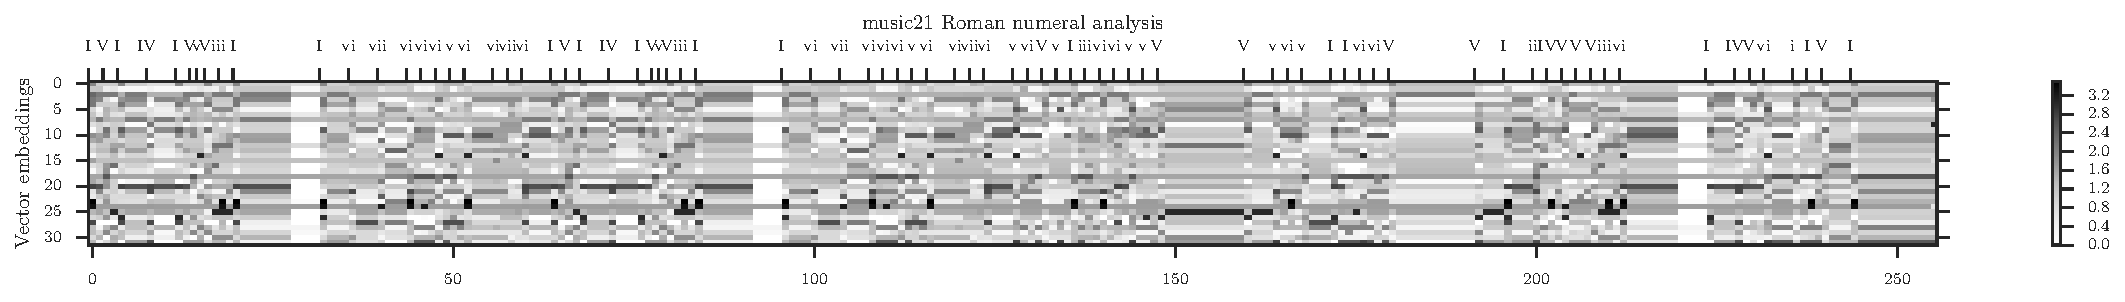
\includegraphics[width=1.0\linewidth]{model-analysis-chords-0.pdf}
    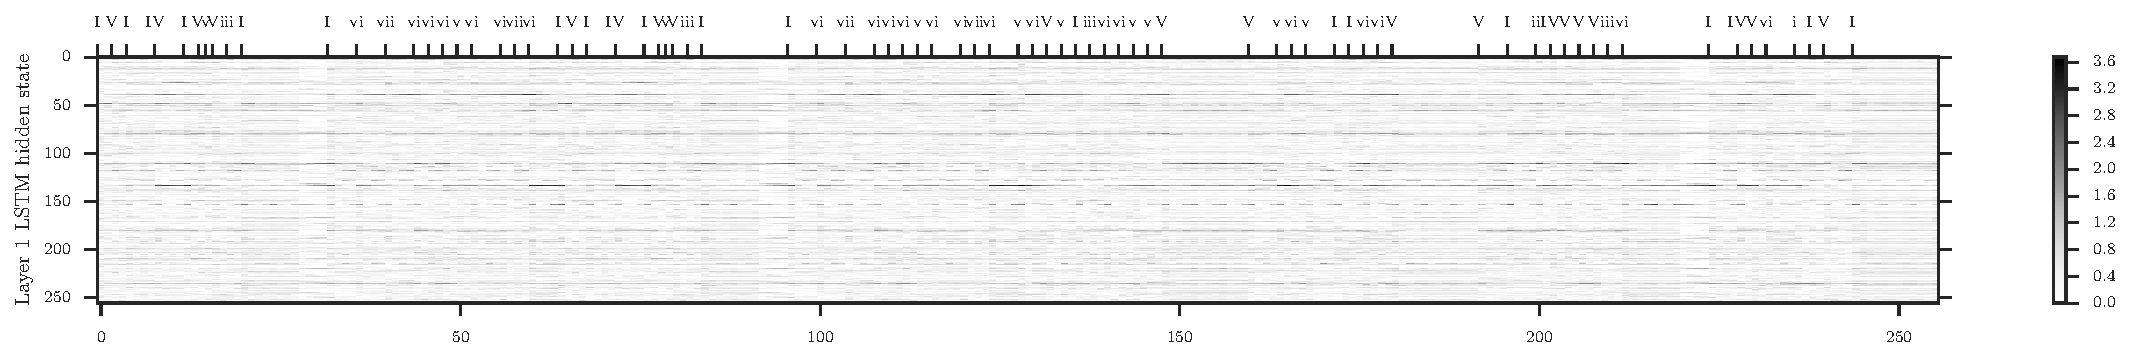
\includegraphics[width=1.0\linewidth]{model-analysis-chords-1.pdf}
    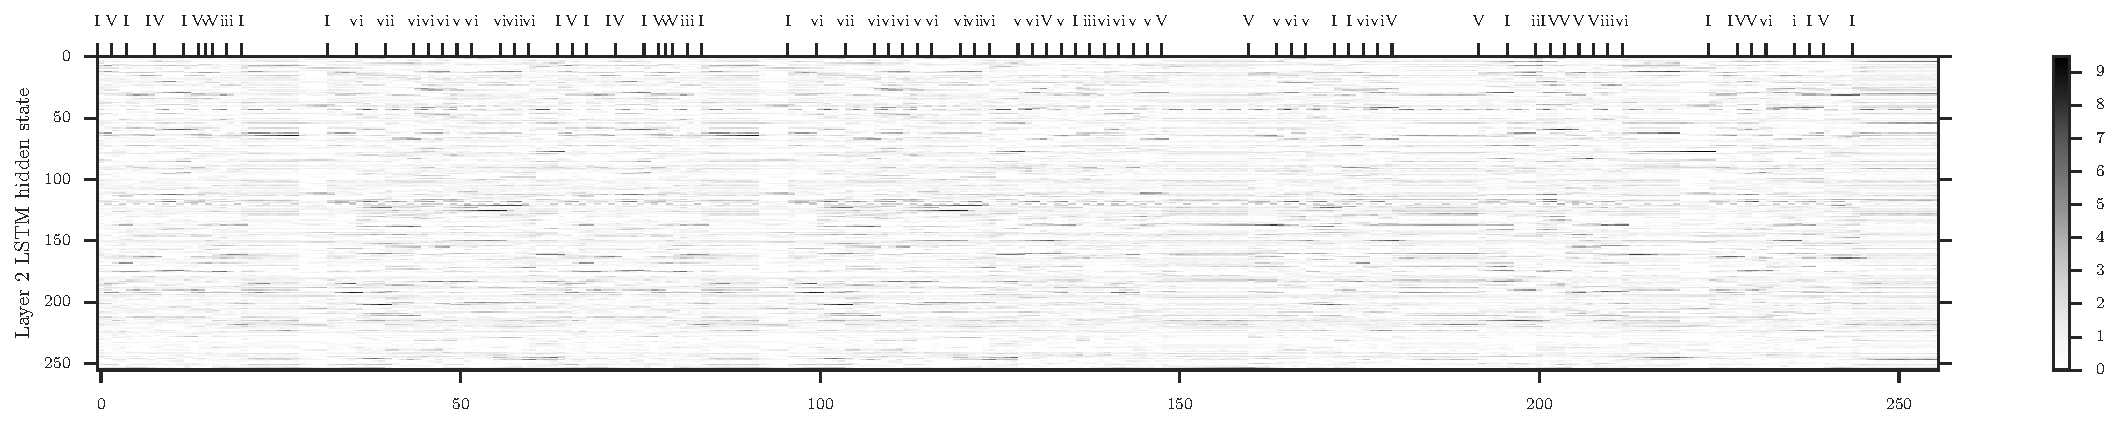
\includegraphics[width=1.0\linewidth]{model-analysis-chords-2.pdf}
    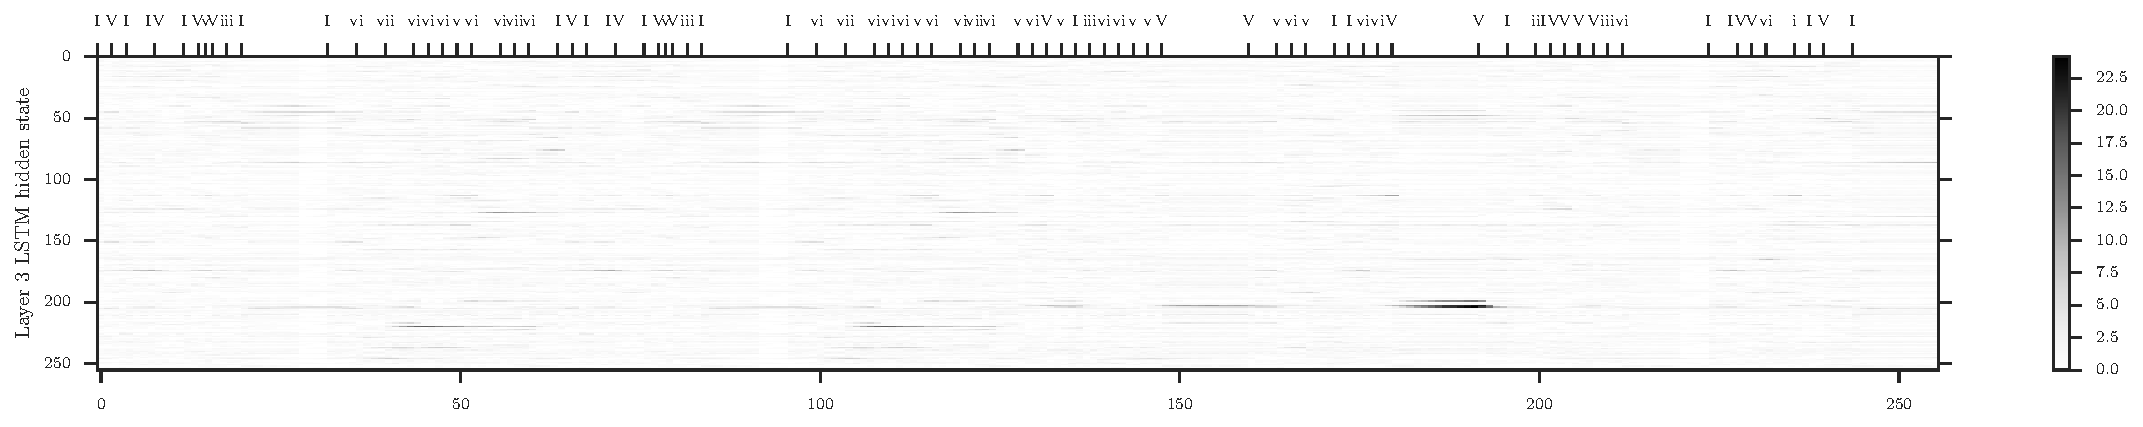
\includegraphics[width=1.0\linewidth]{model-analysis-chords-3.pdf}
    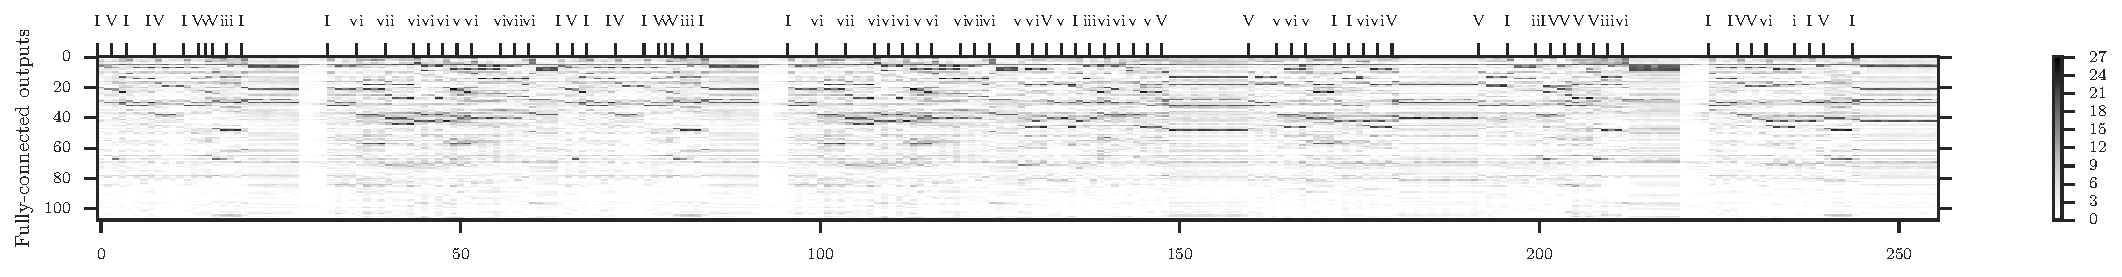
\includegraphics[width=1.0\linewidth]{model-analysis-chords-4.pdf}
    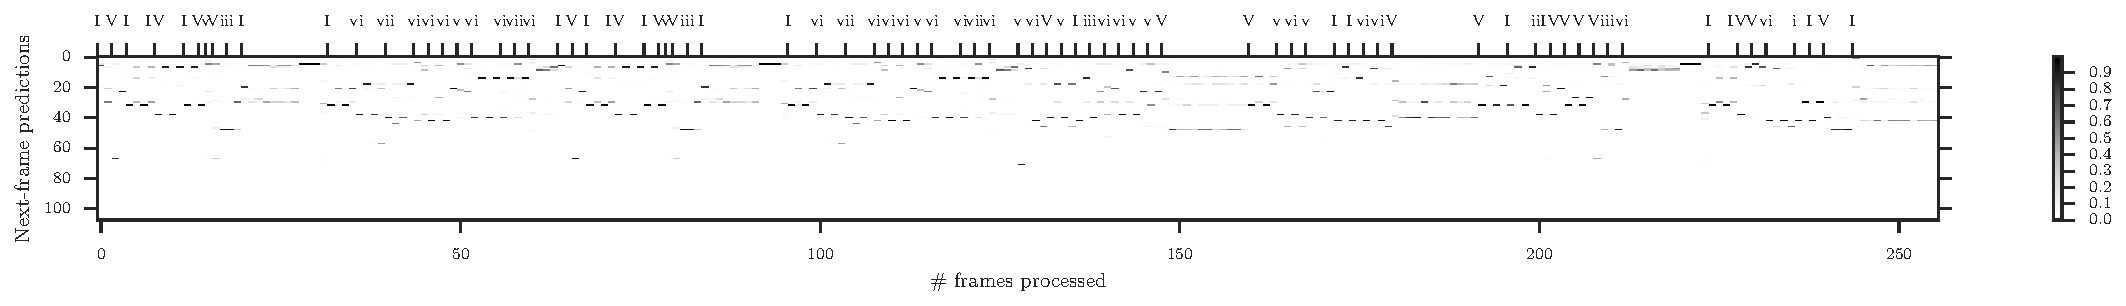
\includegraphics[width=1.0\linewidth]{model-analysis-chords-5.pdf}
    \caption{Neuron activations after max pooling over frames}
    \label{fig:model-analysis-frames}
\end{figure}

The max-pooled frame-level activations are shown in
\cref{fig:model-analysis-frames} As a result of pooling, the horizontal axis
can be aligned and compared against the stimulus
\cref{fig:model-analysis-stimulus}.  This is note the case for unpooled
token-level activations (see \vref{fig:model-analysis-tokens}).

Notice the vertical bands corresponding to when a chord/rest is held for
multiple frames. Also, the vector embedding corresponding to (\eg near frames
$30$ and $90$ in \cref{fig:model-analysis-frames} top) are sparse, showing up
as white smears on the LSTM memory cells at all levels of the model.

\subsection{Probabilistic piano roll: likely variations of the stimulus}

The bottom panel in \cref{fig:model-analysis-frames} shows the model's
predictions for tokens in the next frames, where the tokens are arranged
according to some arbitrary ordering of tokens within the vocabulary. To aid
interpretation, the tokens can be mapped back to their corresponding pitches
and laid out to reconstruct a {\bf probabilistic piano
roll}\citep{eck2008learning} consisting of the model's sequence of next-frame
predictions as it processes the input. This is shown in
\cref{fig:model-analysis-probabilistic-piano-roll}.

\begin{figure}[tb]
    %~~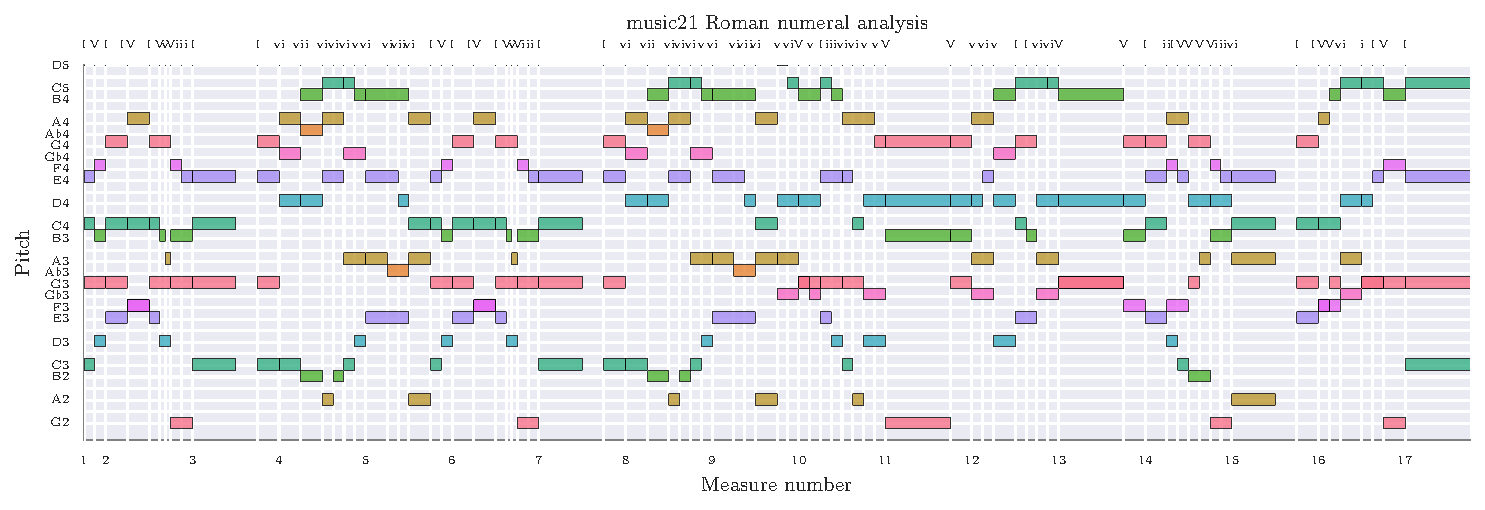
\includegraphics[width=0.99\linewidth]{model-analysis-input-piano-roll.pdf}
    \centering
    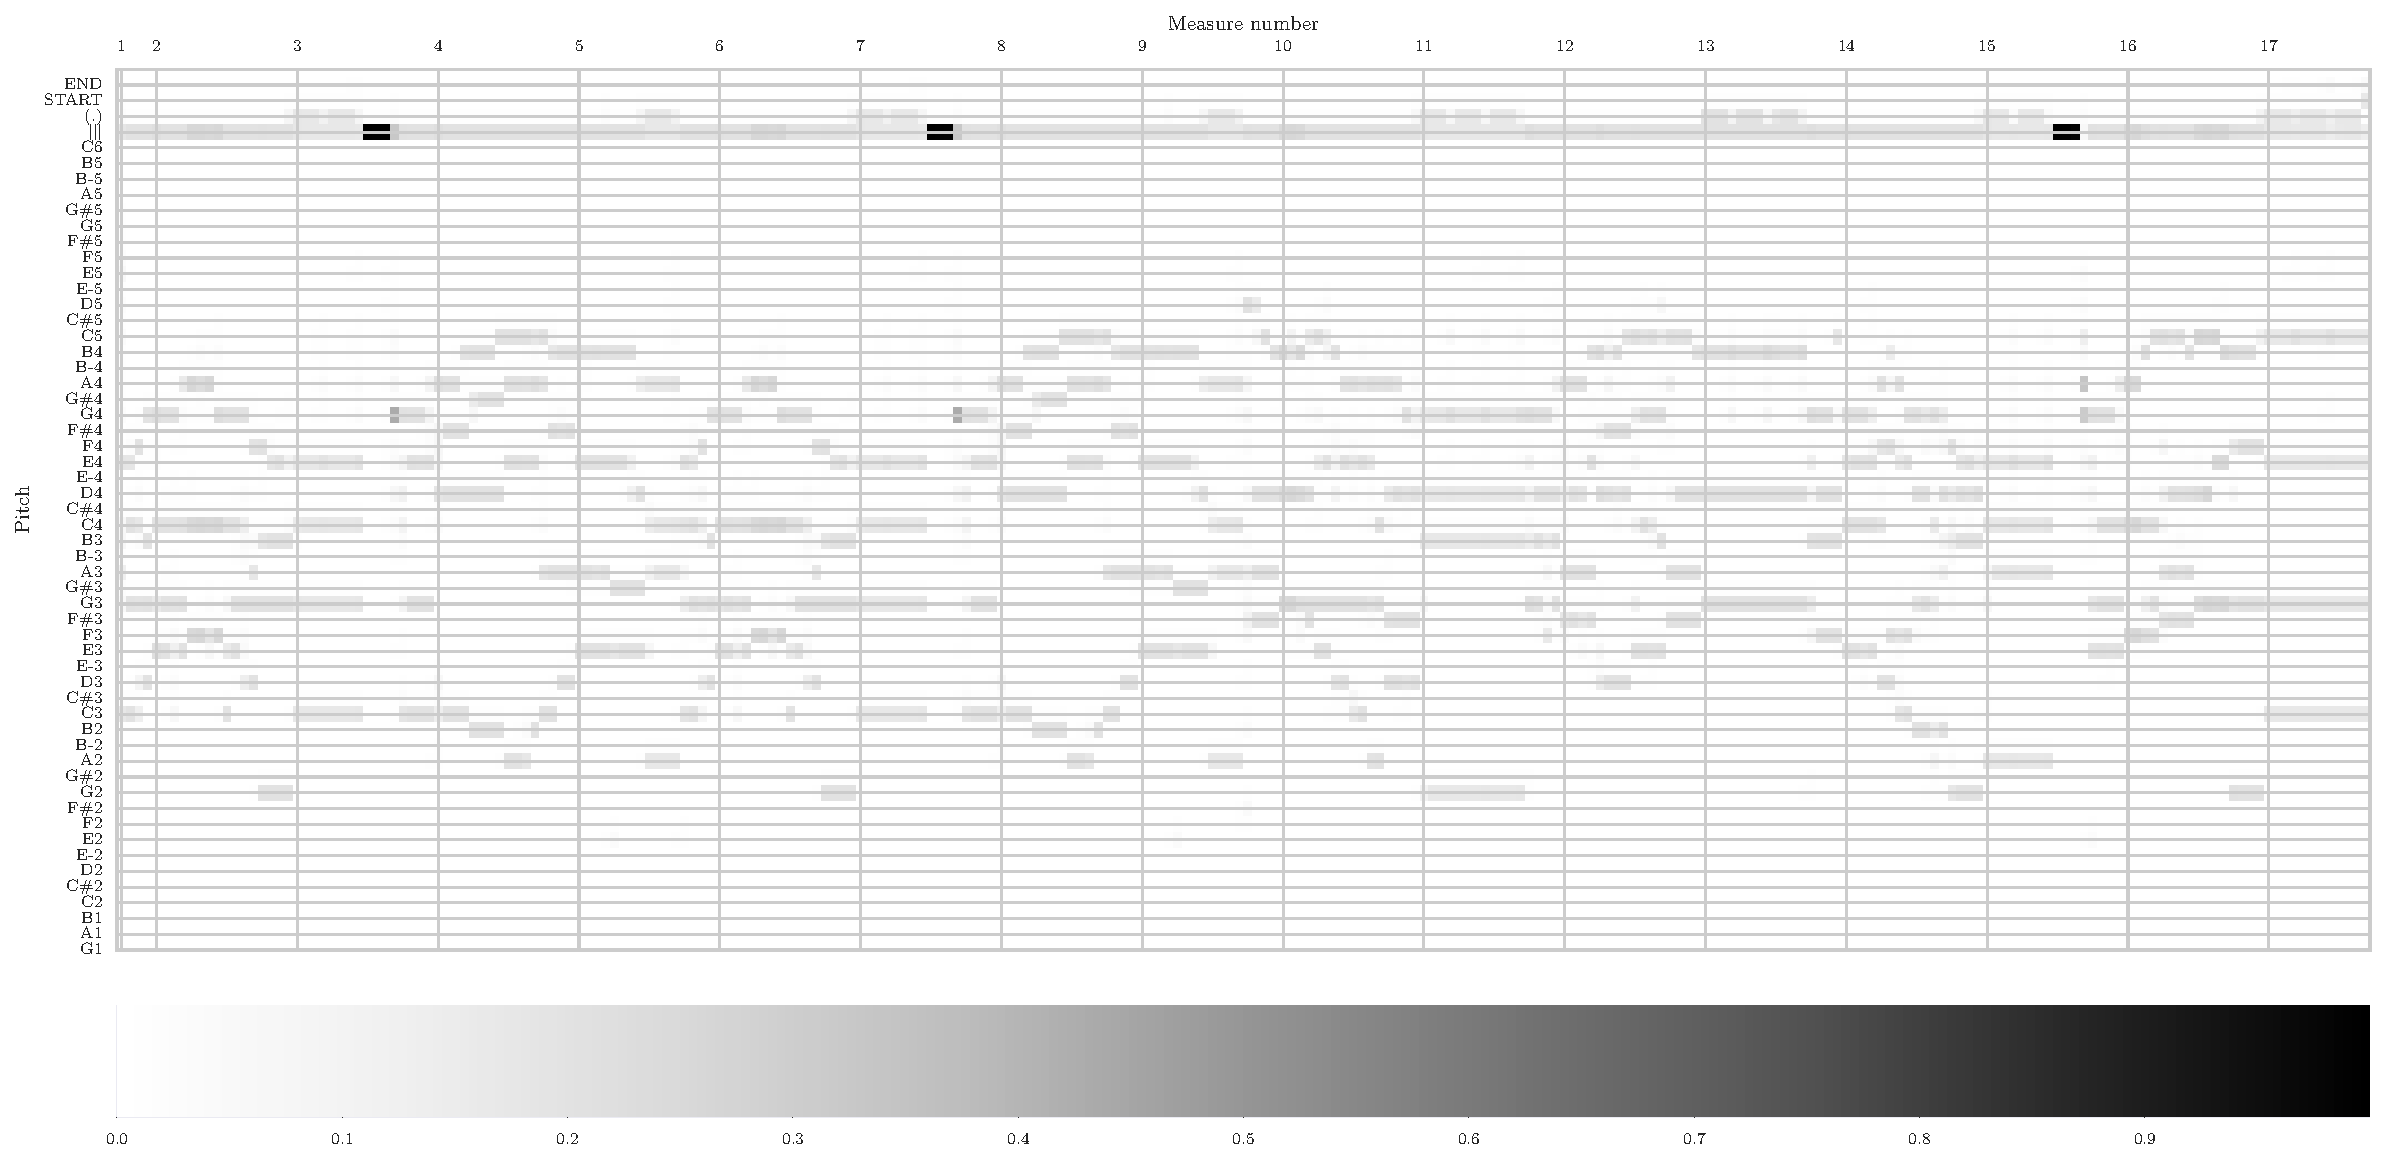
\includegraphics[trim={0 0 0 0},clip,width=1.0\linewidth]{model-analysis-probabilistic-piano-roll.pdf}
    \caption{Probabilistic piano roll of next note predictions.
        The model assigns high probability to fermatas near ends of phrases, suggesting
        an understanding of phrase structure in chorales.}
    \label{fig:model-analysis-probabilistic-piano-roll}
\end{figure}

One surprising insight from \cref{fig:model-analysis-probabilistic-piano-roll}
is the high probability predictions for fermatas (third from top ``(.)'') near
the end of phrases. This could indicate the model has managed to learned a
notion of phrase structure.

Anotering interesting row of \cref{fig:model-analysis-probabilistic-piano-roll}
corresponds to frame delimiters (fourth from top, ``|||''). Notice that the
predictions for frame delimiters are particularly strong during rests. This is
because rests are encoded as empty frames, so the large probability values
indicate that the model has learned to prolong periods of rests. At the end of
rest periods, the model tends to assign probability across a wide range of
notes, suggesting that there are more permissible notes to play at the end of a
rest than in the middle of a phrase. Finally, the probability assigned to
fermatas is larger near the ends of phrases, suggesting that the model has
learned some notion of of phrasing within music.

However, it may also not be very significant. Notice that the probabilistic
piano roll in \cref{fig:model-analysis-probabilistic-piano-roll} closely
resembles the stimulus. This is because the recurrent inputs are taken from the
stimulus rather than sampled from the model's predictions (a.k.a.
\citep{williams1989learning}), so a model which predicts to only continue
holding its input would produce a probabilistic piano roll identical to the
stimulus delayed by one frame.

\subsection{Neurons specific to musical concepts}\label{sec:music-concept-neurons}

Research in convolutional networks has shown that individual neurons within the
network oftentimes specialize and specifically detect certain high-level visual
features \citep{zeiler2010deconvolutional}. Extending the analogy to musical
data, we might expect certain neurons within our learned model to act as
specific detectors to certain musical concepts.

To investigate this further, we look at the activations over time of individual
neurons within the LSTM memory cells. We discover certain neurons whose
activities appear correlated to specific motifs, chord progression, and phrase
structures, and show their activity profiles in
\cref{fig:model-analysis-cells-individual}.

\begin{figure}[tb]
    \centering
    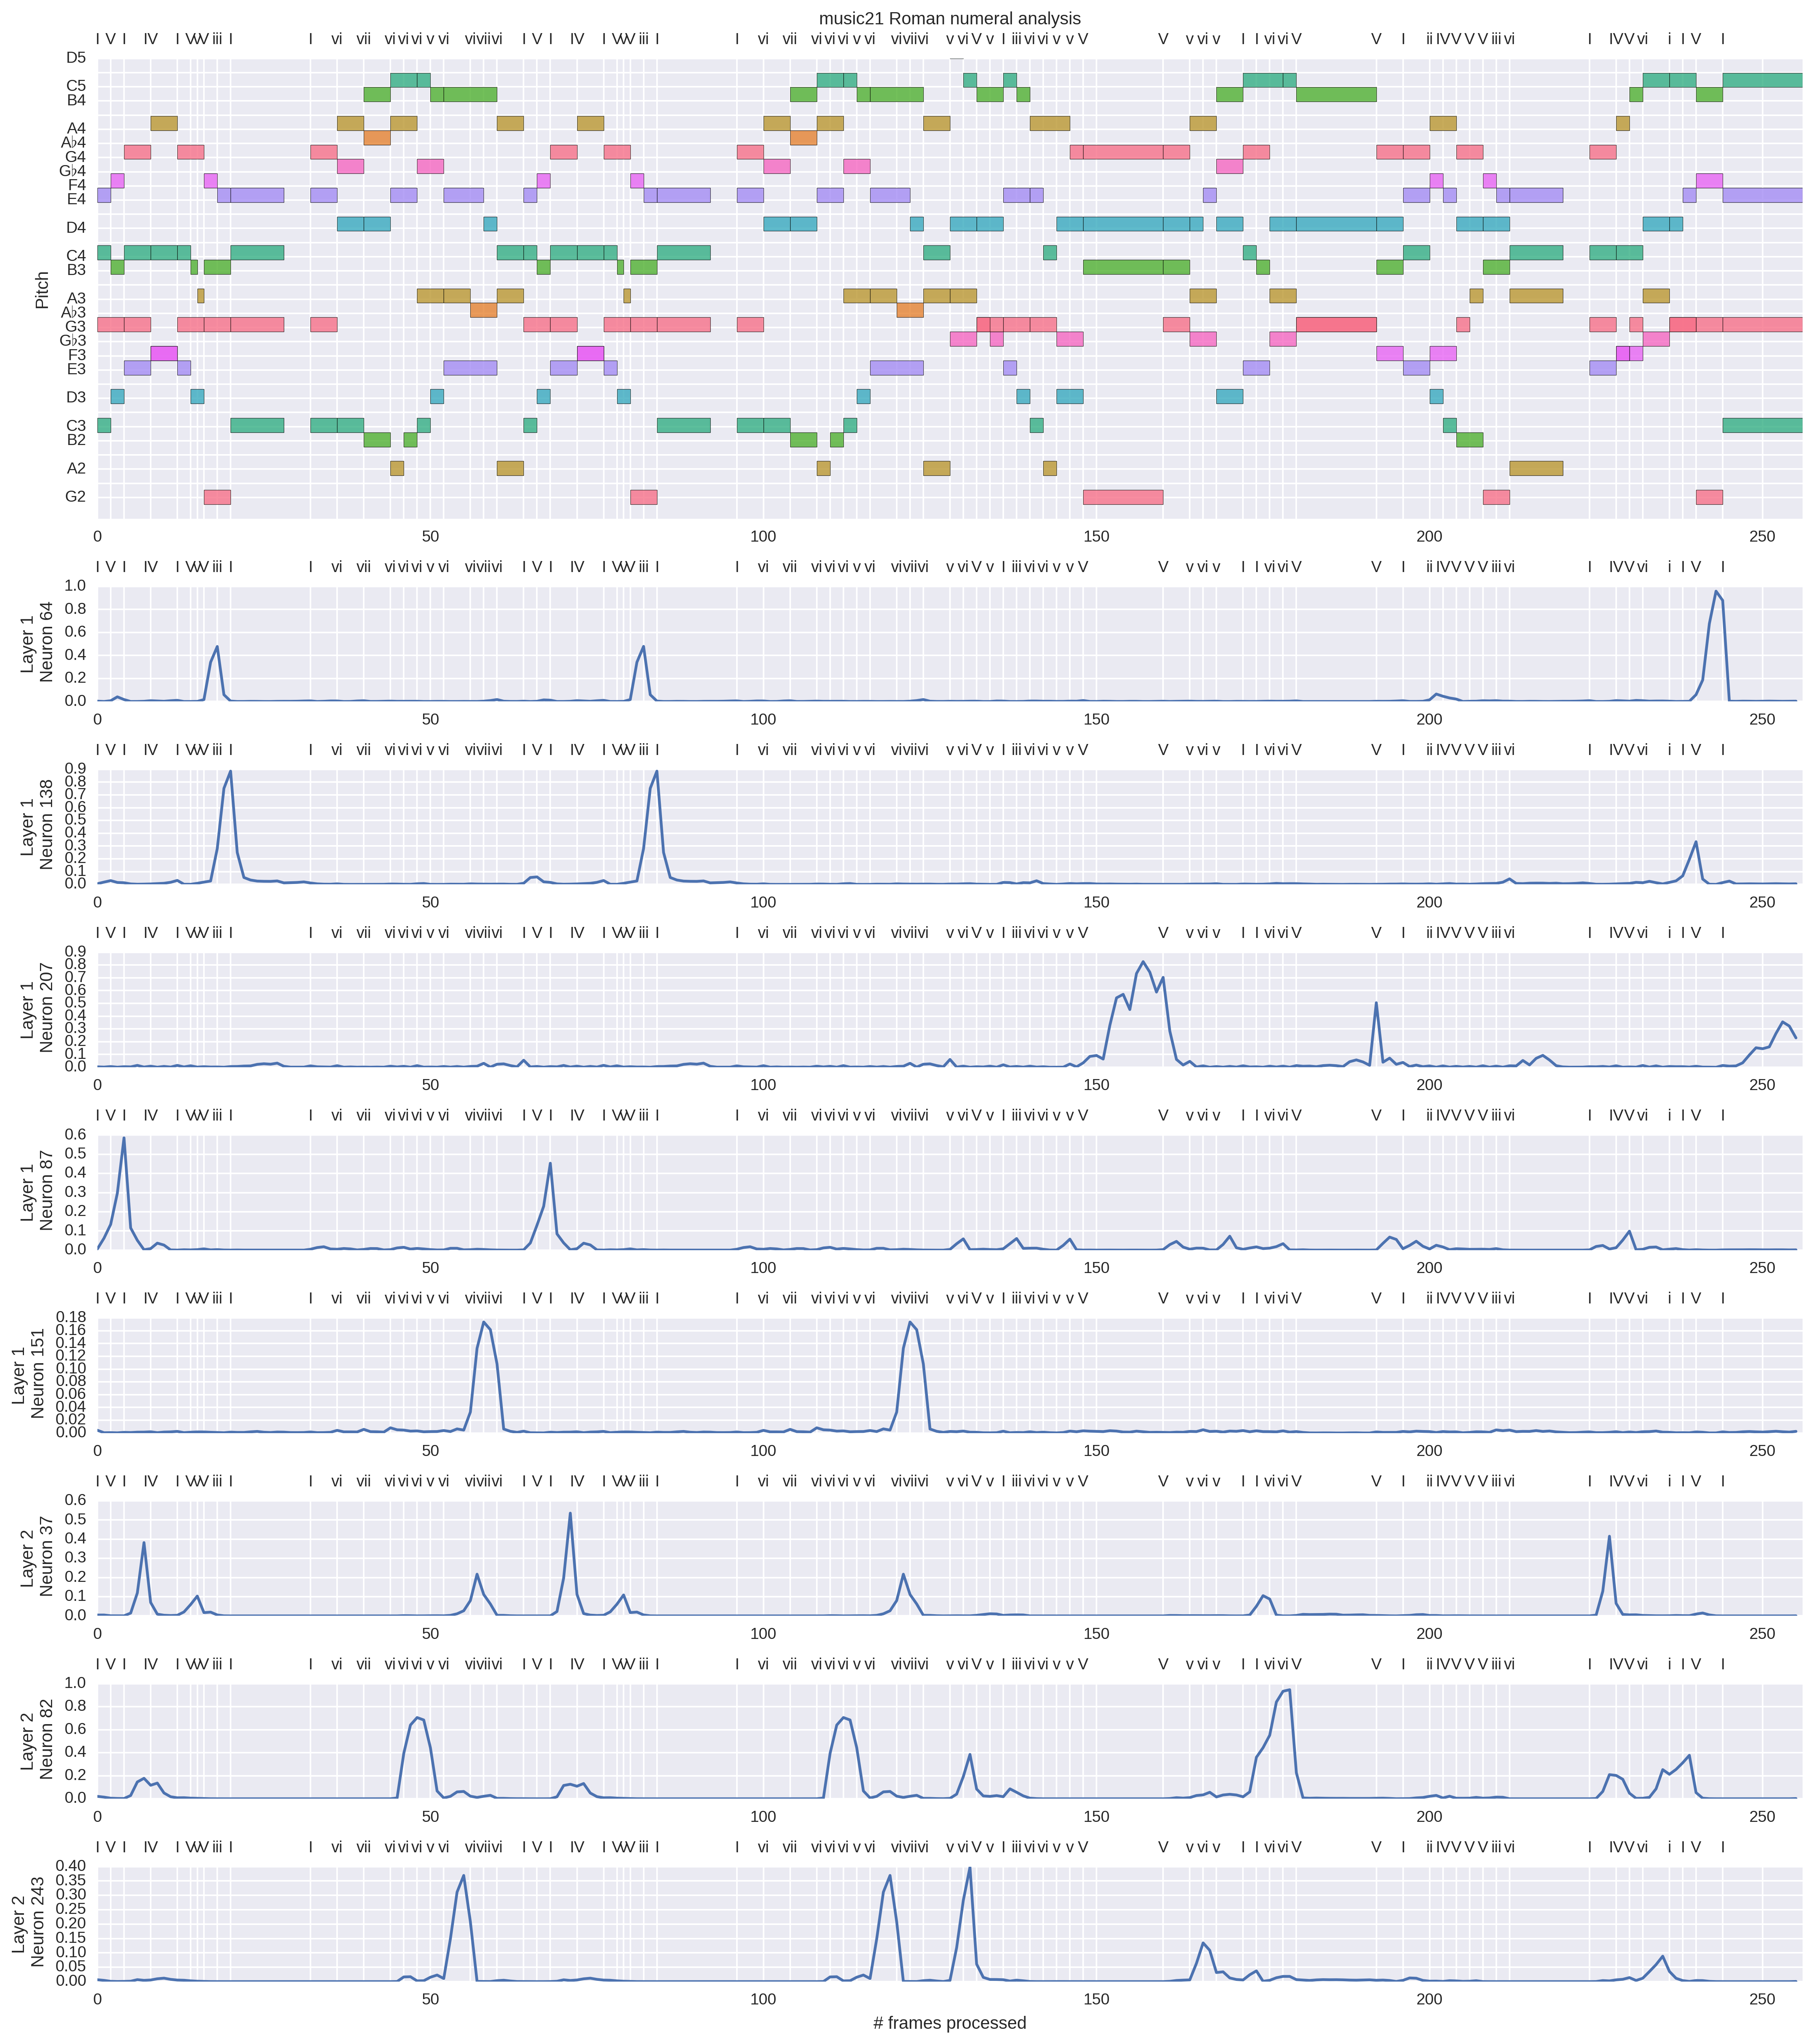
\includegraphics[width=1.0\linewidth]{model-analysis-cells-individual.png}
    \caption{Activation profiles demonstrating that neurons have specialized to become
    highly specific detectors of musically relevant features}
    \label{fig:model-analysis-cells-individual}
\end{figure}

Given our limited knowledge of music theory, we provided the actication
profiles for our collaborator Dr.\ Mark Gotham \citet{mark-analysis}, who
provided the following remarks:
\begin{itemize}
    \item The first two (Layer 1, Neuron 64 / Layer 1, Neuron 138) seem to pick out (specifically) perfect cadence
        with root position chords in the the tonic key.
    \item There are no imperfect cadences here; just one interruptions into bar 14.
    \item Layer 1, Neuron 87: the I$^6$ chords on the first downbeat, and its reprise 4 bars later.
    \item Layer 1, Neuron 151: the two equivalent a minor (originally b minor) cadences that end phrases 2 and 4.
    \item Layer 2, Neuron 37: Seems to be looking for I$^6$ chords: strong peak
        for a full I$^6$; weaker for other similar chords (same bass).
    \item The rest are less clear to me.
\end{itemize}
Dr.\ Gotham's analysis suggests that while some neurons are ambiguous to interpretation,
other neurons have learned highly specific and musically relevant concents.

To our knowledge, this is the first reported result demonstrating LSTM neurons
specializing to detect musically meaningful features. As we were careful to
avoid imposing prior assumptions when designing the model, these neurons
learned to specialize as a result of exposure to the Bach data. While we are
hesitant to make broader conclusions from this single experiment, the
implications of this finding are tremendously exciting for music theorists
and deep learning researchers alike. We propose future work in this area
in \vref{sec:future-work}.

